\documentclass[11pt]{article}

% ---------------------------------------------------------------- packages
\usepackage[margin=1in]{geometry}
\usepackage{amsmath,amssymb}
\usepackage{graphicx}
\usepackage{booktabs}
\usepackage{siunitx}
\usepackage{caption}
\usepackage{subcaption}
\usepackage{authblk}
\usepackage[numbers,sort&compress]{natbib}
\usepackage[hidelinks]{hyperref}
\usepackage{xcolor}
\usepackage{enumitem}
\usepackage{microtype}
\graphicspath{{figures/}}
\captionsetup{font=small,labelfont=bf}
\sisetup{detect-all}

\newcommand{\sharpe}{\ensuremath{\mathrm{SR}}}

% ---------------------------------------------------------------- title
\title{\bfseries Do Candlestick-Image CNNs Predict Crypto Returns?\\
A Pre-Registered, Survivorship-Corrected Replication with\\ Principled Benchmarks}

\author[1]{Author Name}
\affil[1]{Affiliation\\ \texttt{aps9412@gmail.com}}
\date{\today}

\begin{document}
\maketitle

% ================================================================ abstract
\begin{abstract}
\citet{jiang2023reimagining} (JKX) show that a convolutional neural network (CNN) reading a
\emph{picture} of a price chart predicts future US-equity returns. We ask whether the same
architecture transfers to cryptocurrency, a market that trades continuously, carries no
fundamentals, and has a short, survivorship-hostile history. To avoid the usual traps of a
``does deep learning work'' study, the entire design---four image$\times$horizon configurations,
a $365$-day annualization, a four-point cost grid, and a volatility-regime stratification---was
\emph{pre-registered} before any model was trained, and every raw Sharpe ratio is reported only
alongside its multiple-testing correction, its transaction cost, a full benchmark comparison, and
a direct measurement of survivorship bias. On a point-in-time top-100 universe built from Binance
data (2018--2026; out-of-sample 2021--2026), \textbf{two of the four pre-registered configurations
survive Bonferroni correction} (annualized Sharpe $1.47$ and $1.09$, $p=0.002$ and $p=0.044$).
Crucially, because Binance---unlike equity data vendors---retains delisted coins, we can
\emph{measure} rather than assume the survivorship contribution, and find it is essentially zero
for both winners. The CNN beats every benchmark on identical rows: buy-and-hold BTC, equal-weight
top-100, cross-sectional momentum and reversal, the \citet{han2016trend} trend factor, and a
Kalman trend/vol state estimator adapted from a cointegration filter. The signal is nearly
uncorrelated with reversal and carries no market beta, so it is not a known factor in disguise.
A linear model on the same pixels captures much of the five-day signal but little of the twenty-day
one, so the network's value is horizon-dependent, and both surviving configurations clear a
deflated-Sharpe test that corrects for the number of trials and for non-normality. The binding
constraint is economic: under an endogenous, deliberately conservative \citet{corwin2012simple}
spread estimate, only the low-turnover twenty-day configuration remains non-negative, and the
edge's reliance on shorting illiquid coins puts its realizable Sharpe well below its gross value.
We release all code and a forward paper-trading harness.
\end{abstract}

% ================================================================ intro
\section{Introduction}

A striking recent result in empirical asset pricing is that a CNN trained on \emph{images} of
price charts---ordinary open-high-low-close (OHLC) candlesticks with a moving-average overlay and a
volume bar---predicts the sign of future returns, and that a long--short portfolio formed from its
predictions earns a high Sharpe ratio in US equities \citep{jiang2023reimagining}. The network
receives no engineered features, no returns, no fundamentals: only the picture. This is at once
provocative (it suggests exploitable visual structure in prices) and fragile (image-based deep
learning is exactly the kind of high-capacity model that overfits and that invites data-mining).

We ask a deliberately narrow question: \emph{does this architecture transfer to cryptocurrency?}
Crypto is a natural out-of-distribution test. It trades $24/7$ with no market close, has no
earnings or book value to anchor a valuation, exhibits far higher volatility than equities, and its
short history is riddled with delistings, token redenominations, and ticker reuse. If a
chart-image CNN carries a real edge, it should appear in a genuinely different market; if it was an
equities-specific artifact, crypto should expose it.

The scientific hazard in any such study is not writing the model---it is that a sufficiently
flexible model, searched over enough configurations, will always produce \emph{a} good-looking
Sharpe. The contribution of this paper is therefore as much methodological as empirical. We adopt
four disciplines, fixed before estimation:

\begin{enumerate}[leftmargin=1.4em,itemsep=2pt]
\item \textbf{Pre-registration.} The configuration grid (two image sizes $\times$ two horizons),
the annualization convention ($365$), the cost grid, and the regime analysis were frozen in
advance. No sixty-day windows or extra horizons were added after seeing results.
\item \textbf{Multiple-testing correction.} The grid \emph{is} the search; we report Bonferroni-
and Benjamini--Hochberg--corrected verdicts across the family, not the best cell.
\item \textbf{Benchmark comparison.} The CNN is scored against naive, cross-sectional-factor, and
state-space benchmarks on identical rows. A CNN that does not beat buy-and-hold or momentum is not
a result, and we say so.
\item \textbf{Survivorship measurement.} Because Binance retains delisted coins, we quantify the
survivorship contribution directly rather than speculating about its sign---something the equities
literature typically cannot do.
\end{enumerate}

Our findings are positive but bounded. Two of four pre-registered configurations survive the
strictest correction; their edge is not a survivorship artifact and is distinct from known factors;
but it leans on short positions in illiquid alt-coins, so its realizable return is below its
paper Sharpe. We regard the honest, corrected null on two of four cells, and the measured-zero
survivorship bias on the two winners, as results of equal standing to the positive Sharpes.

% ================================================================ related
\section{Related work}

\paragraph{Images of prices.} \citet{jiang2023reimagining} introduce the candlestick-CNN and
document its predictive power and portfolio performance on CRSP data; we replicate their image
encoding and network verbatim. Earlier work encodes prices as Gramian or recurrence images for
classification; JKX's contribution is the OHLC-plus-volume rendering and the portfolio evaluation.

\paragraph{Cross-sectional factors.} Our benchmarks are the canonical price-based predictors:
intermediate-horizon momentum \citep{jegadeesh1993returns}, short-horizon reversal
\citep{jegadeesh1990evidence,lehmann1990fads}, and the moving-average trend factor of
\citet{han2016trend}, which we implement as their fitted cross-sectional forecast rather than a
moving-average crossover vote.

\paragraph{State-space benchmark.} We add a Kalman trend/vol estimator adapted from a
mean-reverting cointegration filter in the spirit of \citet{avellaneda2010statistical}, repurposed
from a two-state hedge-ratio filter into a two-state local-linear-trend filter. This gives the CNN
a \emph{principled} predictor to beat, not merely a naive factor.

\paragraph{Survivorship and replication.} The direction and magnitude of survivorship bias is
notoriously hard to pin down in equities because delisted names are often unavailable. Crypto
inverts this: exchange APIs retain dead tickers, enabling direct measurement. Our insistence on
pre-registration and correction follows the reproducibility critique of factor research
\citep{harvey2016andthecrosssection}.

% ================================================================ data
\section{Data}

\subsection{Source and the survivorship inversion}
We use daily klines from Binance's public data mirror (\texttt{data-api.binance.vision}), which
requires no key. Every claim below was probed empirically. BTCUSDT daily history begins
2017-08-17, and BTCUSDT has a bar on $100.0\%$ of calendar days (3{,}257 of 3{,}257), which is why
we annualize by $365$ throughout rather than by $252$.

The central data finding is that \textbf{crypto inverts the equity survivorship problem}. Equity
vendors purge delisted tickers; in the sibling equities study, $429$ of $703$ de-indexed S\&P names
were unrecoverable and coverage drifted by $+34.9$ percentage points across the out-of-sample
window. Binance instead retains delisted symbols (\texttt{status=BREAK}) with full history: of $701$
USDT pairs, $242$ are dead; of $488$ BTC pairs, $439$ are dead; and $15$ of $15$ sampled dead pairs
(including LUNA, UST, and FTT through their respective collapses) returned complete history.
Consequently the dead coins are both \emph{enumerable} and \emph{retrievable}.
Figure~\ref{fig:data}(a) shows that a large fraction of each early cohort of the traded universe is
now delisted yet remains in the panel.

\subsection{Two disclosed deviations from the pre-registered universe}
Two locked design choices proved infeasible on free data and were amended \emph{before} building,
with the amendments disclosed here.

\emph{(i) Ranking variable.} No free point-in-time market-capitalization source exists (market cap
needs circulating-supply history, which no free API serves; CoinGecko, CoinPaprika, CryptoCompare,
Messari, and CoinMarketCap's historical pages were each probed and rejected). We therefore rank the
universe by \textbf{trailing 30-day median dollar volume} ($\text{Close}\times\text{Volume}$),
lagged one day so it is strictly point-in-time. This is a liquidity rank, not market cap: it
over-weights high-turnover coins. To prevent misreading, the panel carries \emph{no}
\texttt{market\_cap} column.

\emph{(ii) Quote currency.} Binance had only six clean USDT-quoted coins on 2018-01-01 and did not
reach one hundred until mid-2020; it was BTC-quoted in the early period. We therefore take a coin's
USD price from its USDT print when available, else from $\text{coin/BTC}\times\text{BTCUSDT}$. The
cross-rate is exact at the close but approximate for the intraday high/low. Critically, this
approximation is concentrated in the \emph{training} years and is negligible in the reported
out-of-sample window (Figure~\ref{fig:data}(b)): $86.6\%$ of 2018 universe rows are cross-rated,
falling to $\approx\!0.6\%$ from 2021 onward.

\begin{figure}[t]
\centering
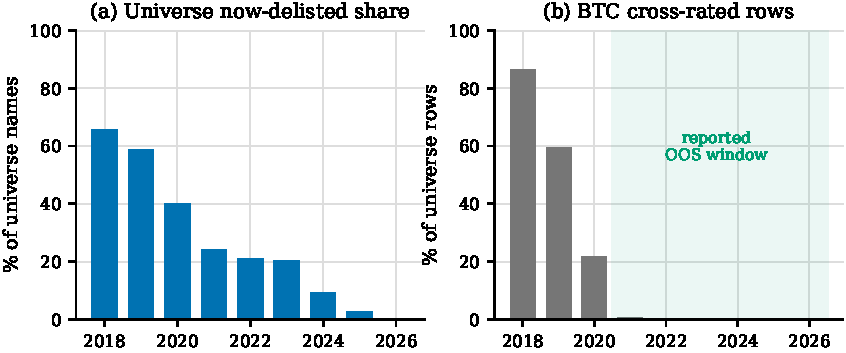
\includegraphics[width=\linewidth]{fig_data.pdf}
\caption{\textbf{Data honesty.} (a) Share of each year's top-100 universe that is delisted as of the
sample end but retained in the panel with full history---the dead coins are present, not missing.
(b) Fraction of universe rows priced via the BTC cross-rate; the approximation is concentrated in
the training years and is negligible in the reported out-of-sample window (shaded).}
\label{fig:data}
\end{figure}

\subsection{Cleaning: two return-fabricating traps}
Raw exchange data contains discontinuities that manufacture enormous fake returns; each was fixed
structurally rather than by clipping returns.

\emph{Ticker reuse.} \texttt{LUNAUSDT} was Terra Classic until its 2022 collapse, then---after an
18-day halt---resumed as Terra 2.0, a different asset on the same ticker. Naively concatenated this
produces a $+177{,}399\times$ one-day ``return.'' We split a symbol into separate assets at any
trading gap exceeding seven days.

\emph{Redenomination.} Binance klines carry no split adjustment. \texttt{COCOS} executed a $1{:}1000$
token swap on 2021-01-23 ($\$0.000695\!\to\!\$0.90$ across a four-day halt, volume $\div 1000$), which
a gap rule alone misses. Across the panel, all eight $>\!5\times$ jumps that coincide with a halt are
units changes (price $\div k$ with volume $\times k$), whereas all eleven consecutive-day jumps are
real market events. We therefore split the series at a $>\!5\times$ jump \emph{spanning a halt} and
never touch consecutive-day moves. This is a units correction, not winsorization: LUNA's $-99.97\%$
and the 2025 MANTRA (\texttt{OM}) $-83.9\%$ crash survive intact, since those are precisely the
collapses a short leg should capture.

\subsection{Leak-free construction and the final panel}
Every forward-looking quantity passes a corruption test: overwriting prices from time $t$ onward
must leave every value dated $\le t$ bit-identical. This holds for the volatility regime (a
30-day return standard deviation lagged to end at $t-1$), the \citet{han2016trend} trend factor
(betas realized only at $t+H$, and rebalance dates spaced exactly $H$ apart), and the dollar-volume
rank. The resulting panel has $887{,}326$ rows over $662$ assets (2018-01-01 to 2026-06-30);
$618$ assets pass through the top-100 universe and $436$ of them ($71\%$) are delisted with full
history retained. The universe holds a mean of exactly $100.0$ names on all $3{,}093$ dates, with no
coverage drift.

% ================================================================ methods
\section{Methodology}

\subsection{Image encoding and network}
For an $n$-day window we render a grayscale OHLC candlestick image (each day three pixels wide: an
open tick on the left, a close tick on the right, a high--low bar centered), a moving-average line,
and a volume bar, at $32\times15$ ($n{=}5$) or $64\times60$ ($n{=}20$) pixels; prices are normalized
to the window's first close. The network is JKX's \texttt{TrendCNN}, reproduced verbatim: stacked
$\text{Conv}(5\times3)\to\text{BatchNorm}\to\text{LeakyReLU}\to\text{MaxPool}(2\times1)$ blocks (two
for $n{=}5$, three for $n{=}20$) with a vertical stride/dilation in the first block, then
$\text{Dropout}(0.5)$ and a linear layer to two logits. \textbf{The network sees only the image}---no
returns, signals, volatility, or regime label.

\subsection{Labels, splits, and training}
The label is $\mathbf{1}\{r_{t\to t+H}>0\}$. The holding period is enforced to be \emph{exactly} $H$
calendar days---a positional offset could otherwise span a gap and be mis-annualized---and offending
samples are dropped. We train on data through 2020-12-31 (a $70/30$ split for early stopping) and
evaluate out-of-sample on 2021-01-01 to 2026-06-30, a split fixed in advance so the cross-rate
approximation falls in the training period. Each configuration is a five-member ensemble (random
initialization, no bagging; Adam, learning rate $10^{-5}$, batch $128$, early stopping with patience
$2$, fp32); test predictions are averaged.

\subsection{Portfolio construction and inference}
At each rebalance date we sort universe coins into deciles on the ensemble probability and hold the
equal-weight top-minus-bottom (D10$-$D1) book for $H$ days, rebalancing every $H$ calendar days so
periods never overlap. The rebalance calendar is built on the continuous grid
(\texttt{date\_range} at frequency $H$D), and all annualization uses $365/H$. Costs are charged as
$2\times\text{bps}$ per rebalance at $\{0,10,25,50\}$ bps per side. Statistical inference uses
(i) a two-sided $t$-test on the period returns, corrected across the four-cell family by
\textbf{Bonferroni} (multiplier $4$) and \textbf{Benjamini--Hochberg} (FDR $5\%$), and (ii) a
stationary block bootstrap ($2000$ resamples) for a Sharpe confidence interval that respects
autocorrelation.

\subsection{Benchmarks}
On identical rows we score: buy-and-hold BTC and equal-weight top-100 (directional, long-only);
momentum (\texttt{MOM}), one-month and one-week reversal (\texttt{STR}, \texttt{WSTR}), and the
\citet{han2016trend} trend factor (\texttt{TREND})---all market-neutral decile books; and a
\textbf{Kalman trend/vol estimator}. The last adapts a mean-reverting cointegration filter into a
local-linear-trend filter: the latent state is $[\text{level},\text{slope}]$ with transition
$A=\left[\begin{smallmatrix}1&1\\0&\phi\end{smallmatrix}\right]$ (the slope damped toward zero at
rate $\phi$, the cointegration filter's reversion made concrete), observation
$\log(\text{close})=\text{level}$, and signal equal to the filtered slope divided by an
exponentially weighted innovation volatility. It is strictly causal and passes the same corruption
test.

% ================================================================ results
\section{Results}

\subsection{The corrected grid}
Table~\ref{tab:grid} and Figure~\ref{fig:grid} report the pre-registered family. Two of four
configurations survive the strictest correction: \textbf{I5/R5} ($\sharpe=1.47$, Bonferroni
$p=0.002$) and \textbf{I20/R20} ($\sharpe=1.09$, Bonferroni $p=0.044$). I5/R5 is the statistically
strongest, with a block-bootstrap $95\%$ Sharpe interval of $[+0.70,+2.33]$; I20/R20 also clears the
bar with a wider interval ($[+0.14,+1.86]$), reflecting its $100$ non-overlapping periods against
I5/R5's $401$.

\begin{table}[t]
\centering
\caption{\textbf{Pre-registered configuration grid, out-of-sample (2021--2026).} The family of four
tests is the search; $p$-values are corrected across it. Two configurations survive Bonferroni.}
\label{tab:grid}
\small
\begin{tabular}{lccccc}
\toprule
Config & Sharpe & $t$-stat & raw $p$ & Bonferroni $p$ & survives BH \\
\midrule
\textbf{I5/R5}   & \textbf{1.473} & 3.45 & 0.0006 & \textbf{0.0022} & yes \\
\textbf{I20/R20} & \textbf{1.086} & 2.54 & 0.0110 & \textbf{0.0440} & yes \\
I20/R5           & 0.783 & 1.84 & 0.0665 & 0.266 & no \\
I5/R20           & 0.108 & 0.25 & 0.801  & 1.000 & no \\
\bottomrule
\end{tabular}
\end{table}

\begin{figure}[t]
\centering
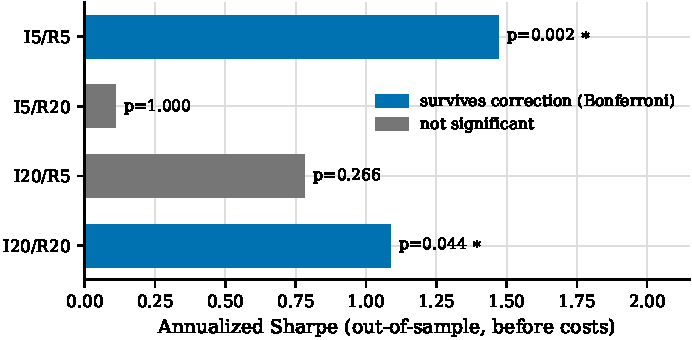
\includegraphics[width=0.82\linewidth]{fig_grid.pdf}
\caption{\textbf{Corrected grid.} Out-of-sample annualized Sharpe by configuration; bars are colored
by whether they survive Benjamini--Hochberg correction, with Bonferroni $p$-values annotated. The
two winners are the ``fast'' (I5/R5) and ``slow'' (I20/R20) diagonal cells.}
\label{fig:grid}
\end{figure}

\subsection{Survivorship: measured, not assumed}
Because dead coins are retained, we decompose each Sharpe by re-introducing the bias---restricting to
coins still trading at the end---and taking the difference (Table~\ref{tab:surv},
Figure~\ref{fig:surv}). \textbf{For both winners the bias is essentially zero} ($-0.00$ for I5/R5,
$-0.21$ for I20/R20). A negative bias means dropping the dead coins \emph{hurts} the strategy: the
CNN correctly profited from coins that later died (e.g.\ by being short as they fell), so a
survivor-selected view understates rather than inflates its edge. The only configuration with a
positive (inflating) bias, I5/R20, is null in any case. This is the measurement the equities
literature usually cannot make.

\begin{table}[t]
\centering
\caption{\textbf{Survivorship decomposition.} ``True point-in-time'' uses the full historical
universe; ``survivors-only'' restricts to coins alive at the sample end. Bias $=$ survivors $-$ true.}
\label{tab:surv}
\small
\begin{tabular}{lccc}
\toprule
Config & True point-in-time \sharpe & Survivors-only \sharpe & Bias \\
\midrule
I5/R5   & 1.473 & 1.472 & $-0.001$ \\
I20/R20 & 1.086 & 0.874 & $-0.213$ \\
I20/R5  & 0.783 & 0.778 & $-0.005$ \\
I5/R20  & 0.108 & 0.426 & $+0.319$ \\
\bottomrule
\end{tabular}
\end{table}

\begin{figure}[t]
\centering
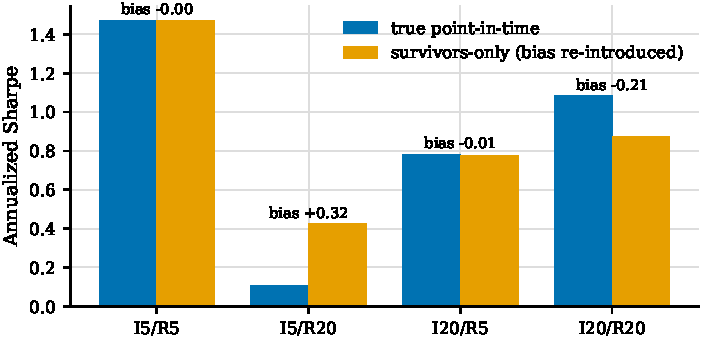
\includegraphics[width=0.72\linewidth]{fig_survivorship.pdf}
\caption{\textbf{Survivorship decomposition.} The two configurations that survive correction have
near-zero (or negative) bias: their edge is not manufactured by dropping delisted coins.}
\label{fig:surv}
\end{figure}

\subsection{Benchmark comparison}
Figure~\ref{fig:bench} and Table~\ref{tab:bench} place the CNN beside every benchmark on identical
rows. Both winners beat every cross-sectional factor \emph{and} the Kalman estimator, gross and at
$25$ bps. The Kalman filter is a genuine opponent (gross $\sharpe=0.71$ at $H{=}5$), so beating it is
a stronger claim than beating naive momentum. Directional benchmarks (buy-and-hold BTC $0.51$;
equal-weight top-100 $0.14$--$0.19$) are shown for context but are not risk-comparable to the
market-neutral books.

\begin{figure}[t]
\centering
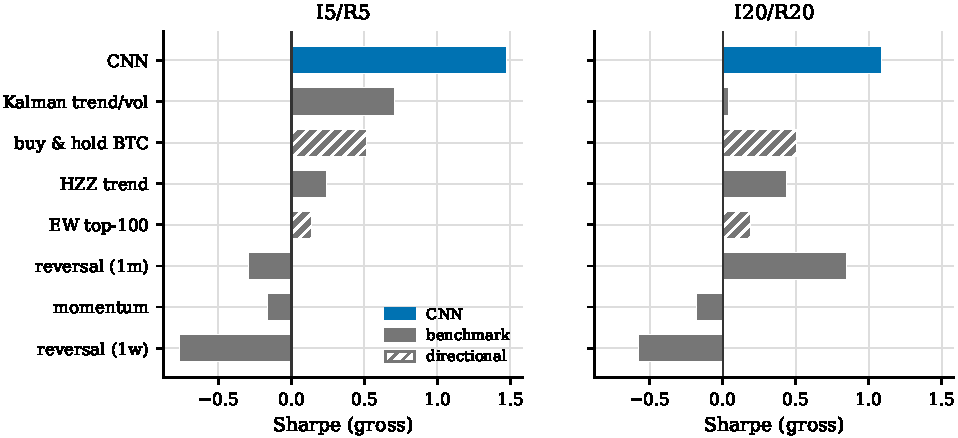
\includegraphics[width=\linewidth]{fig_benchmarks.pdf}
\caption{\textbf{The CNN versus every benchmark}, gross Sharpe, on identical rows. The CNN (blue)
leads in both winning configurations. Hatched bars are directional (long-only) strategies that carry
market beta and are not risk-comparable to the market-neutral books.}
\label{fig:bench}
\end{figure}

\begin{table}[t]
\centering
\caption{\textbf{Benchmark Sharpe ratios} for the two winning configurations, gross and net of the
locked cost grid. MN $=$ market-neutral (long--short); Dir $=$ directional (long-only, charged no
turnover cost).}
\label{tab:bench}
\small
\begin{tabular}{ll cccc c cccc}
\toprule
& & \multicolumn{4}{c}{\textbf{I5/R5}} & & \multicolumn{4}{c}{\textbf{I20/R20}} \\
\cmidrule(lr){3-6}\cmidrule(lr){8-11}
Strategy & Type & 0 & 10 & 25 & 50 & & 0 & 10 & 25 & 50 \\
\midrule
\textbf{CNN}          & MN  & \textbf{1.47} & 1.23 & 0.86 & 0.25 & & \textbf{1.09} & 1.01 & 0.90 & \textbf{0.71} \\
Kalman trend/vol      & MN  & 0.71 & 0.52 & 0.25 & $-0.21$ & & 0.04 & $-0.02$ & $-0.10$ & $-0.23$ \\
Buy \& hold BTC       & Dir & 0.51 & 0.51 & 0.51 & 0.51 & & 0.50 & 0.50 & 0.50 & 0.50 \\
HZZ trend             & MN  & 0.24 & 0.02 & $-0.31$ & $-0.86$ & & 0.43 & 0.37 & 0.28 & 0.12 \\
EW top-100            & Dir & 0.14 & 0.14 & 0.14 & 0.14 & & 0.19 & 0.19 & 0.19 & 0.19 \\
Reversal (1m)         & MN  & $-0.29$ & $-0.46$ & $-0.71$ & $-1.13$ & & 0.85 & 0.79 & 0.70 & 0.55 \\
Momentum              & MN  & $-0.16$ & $-0.37$ & $-0.67$ & $-1.18$ & & $-0.18$ & $-0.23$ & $-0.31$ & $-0.44$ \\
Reversal (1w)         & MN  & $-0.76$ & $-0.95$ & $-1.23$ & $-1.69$ & & $-0.57$ & $-0.62$ & $-0.70$ & $-0.83$ \\
\bottomrule
\end{tabular}
\end{table}

\subsection{Is the CNN a known factor in disguise?}
Sharpe rank alone cannot answer this, so Figure~\ref{fig:corr} correlates the CNN's long--short
return stream with each benchmark's. Both winners are near-uncorrelated with reversal (maximum
$|\rho|=0.38$) and with buy-and-hold BTC ($|\rho|\le0.07$). The CNN is therefore neither repackaged
reversal nor hidden market beta---it is a distinct, genuinely market-neutral signal.

\begin{figure}[t]
\centering
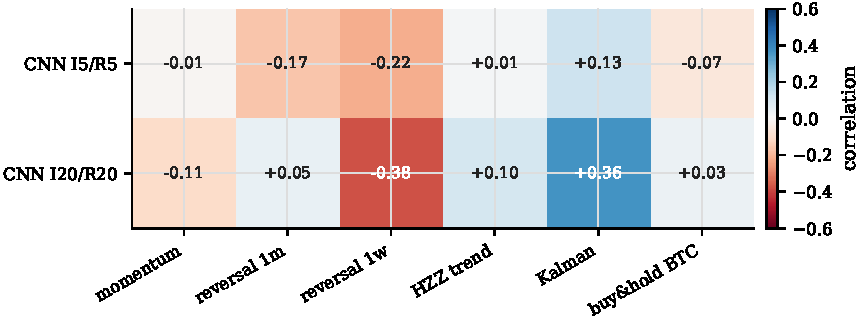
\includegraphics[width=0.85\linewidth]{fig_correlation.pdf}
\caption{\textbf{Return-stream correlations} between the CNN and each benchmark. Low magnitudes
throughout indicate the CNN is distinct from known factors and carries no market beta.}
\label{fig:corr}
\end{figure}

\subsection{Cost sensitivity and the fast/slow trade-off}
Figure~\ref{fig:costs} is the practical crux. I5/R5 has the higher gross Sharpe but decays steeply
with cost (it rebalances every five days), falling to $0.25$ at $50$ bps. I20/R20 rebalances four
times less often and is nearly cost-flat, holding $0.71$ at $50$ bps and overtaking I5/R5 beyond
$\sim\!25$ bps. \textbf{For realistic implementation the slow configuration dominates.}

\begin{figure}[t]
\centering
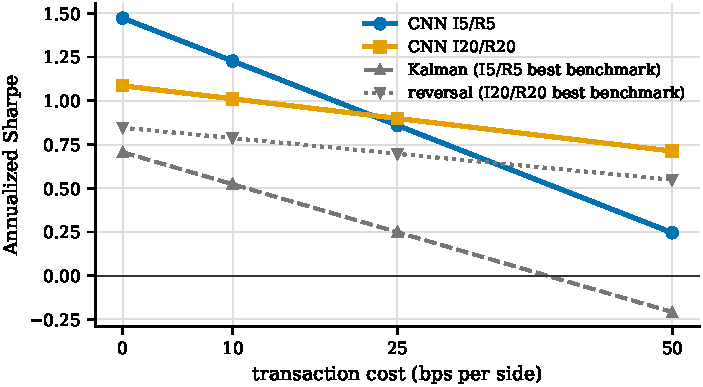
\includegraphics[width=0.72\linewidth]{fig_costs.pdf}
\caption{\textbf{Cost sensitivity.} The fast configuration (I5/R5) starts higher but decays steeply
with turnover; the slow configuration (I20/R20) is nearly cost-flat and dominates beyond $\sim25$ bps.
Benchmarks (gray) are the closest competitor in each config.}
\label{fig:costs}
\end{figure}

\subsection{Structure of the signal}
Figure~\ref{fig:deciles} shows monotonic decile-average returns for I5/R5 (rank correlation
$+0.68$), confirming the signal is coherent across the cross-section rather than driven by a single
tail. However, the extreme deciles are asymmetric: the bottom decile (shorted) averages $-65$ bps
while the top (held long) averages $+55$ bps, and the short leg's stand-alone Sharpe ($1.56$)
exceeds the long leg's ($0.80$). The edge leans on shorting the coins the CNN dislikes.
Figure~\ref{fig:equity} shows the net-of-cost cumulative equity: both winners compound to roughly
five- to eight-fold over the out-of-sample window while remaining decorrelated from BTC's own path.

\begin{figure}[t]
\centering
\begin{subfigure}{0.49\linewidth}
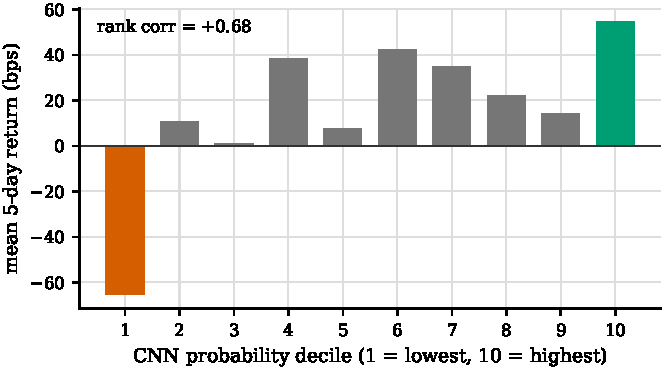
\includegraphics[width=\linewidth]{fig_deciles.pdf}
\caption{}\label{fig:deciles}
\end{subfigure}\hfill
\begin{subfigure}{0.49\linewidth}
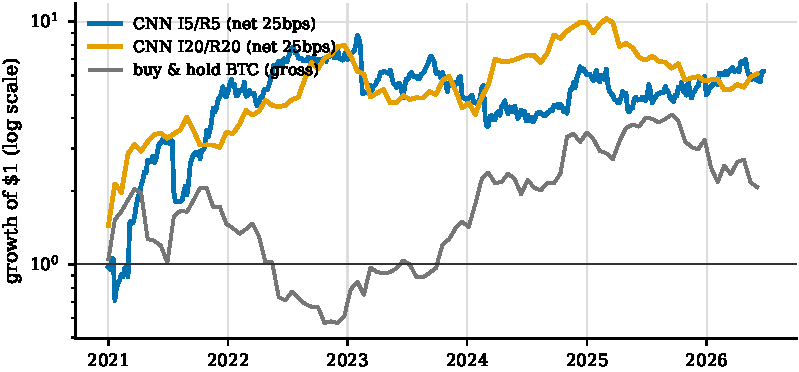
\includegraphics[width=\linewidth]{fig_equity.pdf}
\caption{}\label{fig:equity}
\end{subfigure}
\caption{\textbf{Signal structure.} (a) Decile-average five-day returns for I5/R5 rise monotonically
(rank correlation $+0.68$); the shorted bottom decile is the largest single contributor. (b)
Net-of-cost ($25$ bps) cumulative growth of \$1 for both winners versus gross buy-and-hold BTC.}
\end{figure}

% ================================================================ robustness
\section{Robustness}
\label{sec:robust}

Table~\ref{tab:robust} collects a battery of stress tests on the two surviving configurations. Two
sharpen the case for the model and one substantially tempers its economic claim; we report all three
with equal prominence.

\subsection{Is the deep network necessary?}
We train a logistic regression and gradient-boosted trees \citep{ke2017lightgbm} on the \emph{same}
pixels, labels, and split, and score them identically (Figure~\ref{fig:ablation}). The answer is
\emph{horizon-dependent}. At the five-day horizon a linear model already earns $\sharpe=1.03$ and the
trees $1.20$, against the CNN's $1.47$: much of the short-term signal is linearly decodable from the
image, and the network adds a real but modest increment. At the twenty-day horizon the picture
inverts---logistic $0.21$, trees $0.34$, CNN $\mathbf{1.09}$: the slower pattern is genuinely
nonlinear and the deep architecture is \emph{necessary}, not decorative. Deep learning earns its keep
precisely where a simple model fails.

\subsection{Endogenous transaction costs}
We replace the flat cost grid with a per-coin effective spread estimated from daily high and low
prices via the \citet{corwin2012simple} estimator, charging each traded coin its own round-trip
spread (Figure~\ref{fig:netcost}). This estimator is known to be \emph{upward-biased} for volatile
assets---it attributes part of the intraday range to the spread---so for crypto it is a deliberately
\emph{conservative} (upper-bound) cost: it assigns even BTC a $71$ bps proxy against a true spread of
a few bps, and a universe median of $139$ bps round-trip. Under this stringent assumption the fast
configuration is destroyed by its turnover ($\sharpe$ from $+1.47$ gross to $-1.48$ net), while the
slow configuration remains barely non-negative ($+1.09\to+0.05$). The truth lies between the
flat-$25$-bps net ($0.86$/$0.90$) and this conservative bound; the honest reading is that only the
low-turnover twenty-day configuration is economically plausible, and even it is marginal once
realistic spreads on illiquid coins are paid.

\subsection{Deflated Sharpe, tails, and further checks}
The \citet{bailey2014deflated} Deflated Sharpe Ratio corrects for the number of trials, skewness,
kurtosis, and track length simultaneously. Both winners clear a high bar (probability the Sharpe is
genuine: $0.91$ for I5/R5, $0.96$ for I20/R20), with I20/R20 above the conventional $0.95$ threshold.
The gap reflects tail risk: I5/R5 has extreme excess kurtosis ($24.8$) whereas I20/R20 is milder
($4.5$); both are positively skewed (right-tailed) but carry large maximum drawdowns ($-58\%$ and
$-49\%$ net of $25$ bps), so these are high-risk books despite their Sharpes. Three further checks:
(i) assigning delisted coins their terminal return instead of dropping the window leaves both Sharpes
\emph{identical} ($1.47$, $1.09$), closing the return-level survivorship objection; (ii) the result is
robust in sign and magnitude to the decile count ($5$/$10$/$20$), the minimum cross-section, and a
top-$50$ universe (which weakens both to $\approx\!0.66$, as expected from reduced breadth); and
(iii) all five ensemble members are individually positive ($0.51$ to $1.60$), so no single seed drives
the result. Finally, removing the alt-coin short---holding the top decile long-only, or hedging it
with a short BTC position (the one liquid short)---cuts the Sharpe to $0.45$/$0.31$ and $0.18$/$0.06$
respectively, quantifying how much of the edge is short-side and, therefore, hard to capture.

\begin{table}[t]
\centering
\caption{\textbf{Robustness summary} for the two surviving configurations. Ablation and gross Sharpes
are before costs; ``flat $25$'' and ``Corwin--Schultz'' are net of the respective cost model; DSR is
the deflated-Sharpe probability. All Sharpes annualized at $365/H$.}
\label{tab:robust}
\small
\begin{tabular}{lcc}
\toprule
& \textbf{I5/R5} & \textbf{I20/R20} \\
\midrule
CNN Sharpe (gross)                 & 1.47 & 1.09 \\
\quad gradient-boosted trees, same pixels & 1.20 & 0.34 \\
\quad logistic (linear), same pixels      & 1.03 & 0.21 \\
Deflated Sharpe (prob.\ genuine)   & 0.91 & 0.96 \\
Net, flat $25$ bps/side            & 0.86 & 0.90 \\
Net, Corwin--Schultz (conservative)& $-1.48$ & 0.05 \\
Long-only (directional)            & 0.45 & 0.31 \\
Long D10 / short BTC (tradeable)   & 0.18 & 0.06 \\
Max drawdown (net $25$ bps)        & $-58\%$ & $-49\%$ \\
Sortino (net $25$ bps)             & 1.08 & 1.94 \\
Ensemble-member Sharpe s.d.        & 0.31 & 0.24 \\
\bottomrule
\end{tabular}
\end{table}

\begin{figure}[t]
\centering
\begin{subfigure}{0.49\linewidth}
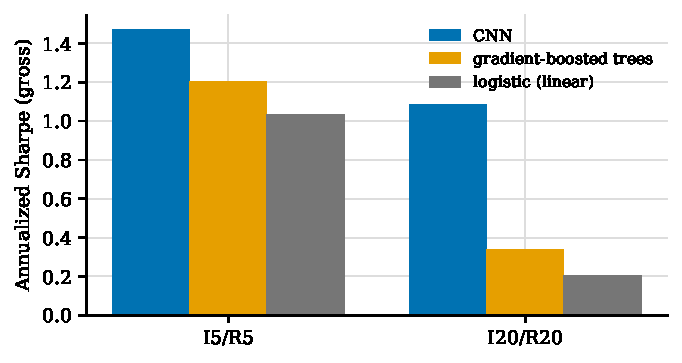
\includegraphics[width=\linewidth]{fig_ablation.pdf}
\caption{}\label{fig:ablation}
\end{subfigure}\hfill
\begin{subfigure}{0.49\linewidth}
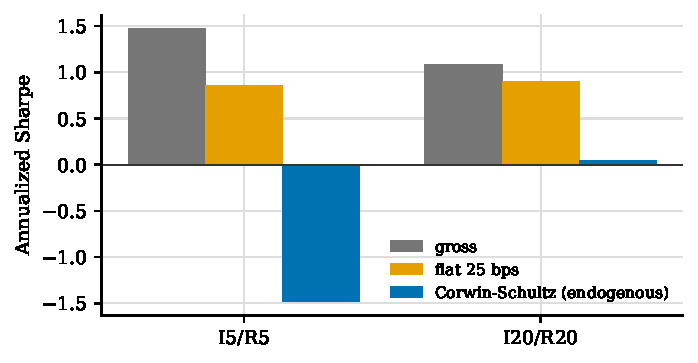
\includegraphics[width=\linewidth]{fig_netcost.pdf}
\caption{}\label{fig:netcost}
\end{subfigure}
\caption{\textbf{Robustness.} (a) The CNN versus a logistic regression and gradient-boosted trees on
identical pixels: the deep network is decisive at the twenty-day horizon but only incremental at five
days. (b) Net Sharpe under a flat $25$ bps cost and under the endogenous, conservative
Corwin--Schultz spread: only the low-turnover configuration survives realistic costs.}
\end{figure}

% ================================================================ discussion
\section{Interpretation: what happened, and why}

\paragraph{Why two of four, and why the diagonal.} The two survivors are the ``matched'' cells
where the image horizon equals the prediction horizon (I5/R5 and I20/R20); the ``mismatched''
off-diagonal cells (I5/R20, I20/R5) fail. A five-day image summarizes very recent price action and
is informative about the next five days but not the next twenty; a twenty-day image captures a
slower pattern suited to a twenty-day forecast. The CNN appears to read structure whose
\emph{timescale matches the image window}, which is why matching the horizon to the window matters
and why a single image size is not universally best.

\paragraph{Why the edge is short-side and cost-sensitive.} The signal's power concentrates in the
bottom decile (Figure~\ref{fig:deciles}): the CNN is better at flagging coins about to fall than
coins about to rise. This is economically intuitive in crypto, where sharp drawdowns and failed
pumps are visually distinctive on a chart, and it explains the cost profile---capturing that
short-side edge requires frequent turnover in exactly the illiquid names that are costly to trade.
The fast cell earns more gross precisely because it re-reads the short-term picture often, and loses
most of it to cost; the slow cell trades a slower, cheaper pattern and survives.

\paragraph{Why it is not just reversal.} Short-horizon reversal is the obvious null hypothesis for
``a model that shorts recent movers,'' but the correlations (Figure~\ref{fig:corr}) refute it: the
CNN's returns are near-orthogonal to both one-week and one-month reversal, and it beats them
outright. The network is evidently conditioning on richer visual structure---candlestick shapes,
the moving-average relationship, volume---than a single past-return sort encodes.

\paragraph{Why survivorship does not explain it.} A skeptic's first reflex is that a long--short
crypto book profits from coins that died. It does---but we \emph{keep} those coins, so that profit is
legitimate and in-sample to the point-in-time universe. Removing them (the survivors-only column)
barely changes I5/R5 and \emph{lowers} I20/R20, demonstrating that the edge is not an artifact of a
survivor-selected universe but, if anything, is understated by one.

% ================================================================ limits
\section{Limitations}

\begin{enumerate}[leftmargin=1.4em,itemsep=2pt]
\item \textbf{Listing survivorship (residual, unfixable from free data).} Our universe is ``top 100
that Binance listed,'' not ``top 100 of all crypto.'' Coins that died on a decentralized exchange or
a competitor before a Binance listing never enter; they skew to losers, so their absence mildly
flatters the long--short book. This is the one bias we can name but not remove.
\item \textbf{Short-leg tradeability---the binding constraint.} The edge is short-concentrated, and
shorting small alt-coins is expensive or infeasible (borrow may not exist). Section~\ref{sec:robust}
quantifies this: under a conservative endogenous spread only the low-turnover configuration is
non-negative, and removing the alt-coin short cuts the Sharpe to $0.31$ (long-only) or $0.06$ (hedged
with a liquid BTC short). The signal is statistically genuine; its \emph{economic} viability is
marginal and hinges on execution.
\item \textbf{Liquidity rank $\ne$ market cap}, and \textbf{cross-rate approximation} in 2018--19
(concentrated in training). Both are disclosed and bounded above.
\item \textbf{Two winners on one market.} This is a single-exchange, single-market study; external
validity to other venues and to a true all-crypto universe is untested.
\end{enumerate}

% ================================================================ conclusion
\section{Conclusion}

Applied to cryptocurrency under a pre-registered, survivorship-corrected, benchmark-anchored
protocol, the JKX candlestick-CNN produces a \emph{statistically} genuine cross-sectional signal in
two of four frozen configurations. The edge survives Bonferroni and deflated-Sharpe correction, is
not a survivorship artifact (measured directly, a luxury crypto affords), beats buy-and-hold,
momentum, reversal, a fitted trend factor, and a Kalman state estimator, is distinct from all of
them, and---at the twenty-day horizon---requires the deep architecture, which a linear model on the
same pixels cannot match. Its limitation is \emph{economic}. The signal is short-concentrated, and
under a conservative endogenous spread estimate only the low-turnover twenty-day configuration
remains non-negative; the tradeable, no-alt-short variants are weakly positive at best. The honest
verdict is therefore a genuine but fragile signal: real enough to reject the null of ``chart images
carry nothing,'' but not yet demonstrated to be net-profitable after the frictions of shorting
illiquid coins. We regard the corrected nulls on the other two cells, the measured-zero survivorship
bias, and the negative cost verdict on the fast configuration as findings on equal footing with the
positive Sharpes. All data-construction code, the training and evaluation notebooks, the robustness
battery, and a forward paper-trading harness are released for replication.

% ================================================================ repro
\section*{Reproducibility}
The pipeline comprises \texttt{crypto\_data\_prep.ipynb} (universe, cleaning, leak-free features),
\texttt{crypto\_train.ipynb} (image store, CNN, corrected grid, survivorship decomposition),
\texttt{crypto\_benchmarks.ipynb} (all benchmarks and correlations), and
\texttt{crypto\_paper\_trade.ipynb} (a forward simulation that trains and saves a production
ensemble, walks the rebalance grid on out-of-sample data, and emits a live target book). All figures
in this paper are generated from the released result files by \texttt{make\_figures.py}.

% ================================================================ refs
\begin{thebibliography}{9}
\bibitem[Avellaneda and Lee(2010)]{avellaneda2010statistical}
M.~Avellaneda and J.-H. Lee.
\newblock Statistical arbitrage in the U.S. equities market.
\newblock \emph{Quantitative Finance}, 10(7):761--782, 2010.

\bibitem[Bailey and L\'opez de Prado(2014)]{bailey2014deflated}
D.~H. Bailey and M.~L\'opez de Prado.
\newblock The deflated Sharpe ratio: Correcting for selection bias, backtest overfitting, and
non-normality.
\newblock \emph{Journal of Portfolio Management}, 40(5):94--107, 2014.

\bibitem[Corwin and Schultz(2012)]{corwin2012simple}
S.~A. Corwin and P.~Schultz.
\newblock A simple way to estimate bid-ask spreads from daily high and low prices.
\newblock \emph{Journal of Finance}, 67(2):719--760, 2012.

\bibitem[Han et al.(2016)]{han2016trend}
Y.~Han, G.~Zhou, and Y.~Zhu.
\newblock A trend factor: Any economic gains from using technical information?
\newblock \emph{Journal of Financial Economics}, 122(2):352--375, 2016.

\bibitem[Ke et al.(2017)]{ke2017lightgbm}
G.~Ke, Q.~Meng, T.~Finley, et~al.
\newblock LightGBM: A highly efficient gradient boosting decision tree.
\newblock \emph{Advances in Neural Information Processing Systems}, 30, 2017.

\bibitem[Harvey et al.(2016)]{harvey2016andthecrosssection}
C.~R. Harvey, Y.~Liu, and H.~Zhu.
\newblock $\ldots$ and the cross-section of expected returns.
\newblock \emph{Review of Financial Studies}, 29(1):5--68, 2016.

\bibitem[Jegadeesh(1990)]{jegadeesh1990evidence}
N.~Jegadeesh.
\newblock Evidence of predictable behavior of security returns.
\newblock \emph{Journal of Finance}, 45(3):881--898, 1990.

\bibitem[Jegadeesh and Titman(1993)]{jegadeesh1993returns}
N.~Jegadeesh and S.~Titman.
\newblock Returns to buying winners and selling losers.
\newblock \emph{Journal of Finance}, 48(1):65--91, 1993.

\bibitem[Jiang et al.(2023)]{jiang2023reimagining}
J.~Jiang, B.~T. Kelly, and D.~Xiu.
\newblock (Re-)Imag(in)ing price trends.
\newblock \emph{Journal of Finance}, 78(6):3193--3249, 2023.

\bibitem[Lehmann(1990)]{lehmann1990fads}
B.~N. Lehmann.
\newblock Fads, martingales, and market efficiency.
\newblock \emph{Quarterly Journal of Economics}, 105(1):1--28, 1990.
\end{thebibliography}

\end{document}
